\documentclass[10pt]{beamer}
\usetheme[background=light,block=fill,progressbar=foot]{metropolis}


%% ctex configuration. slow compiling, comment unless using Chinese.
%\usepackage[UTF8]{ctex}
%\ctexset{refname=References}
%%

\usepackage{graphicx}
\usepackage{caption}
\usepackage{bm}
\usepackage{booktabs}
\usepackage{natbib}
\usepackage{algorithm}
\usepackage{algorithmic} 
\usepackage{transparent}
\newcommand{\supercite}[1]{\textsuperscript{\textsuperscript{\cite{#1}}}}
\newcommand{\emoji}[1]{\text{\raisebox{-0.2em}{\includegraphics[height=1em]{emojis/#1.png}}}}
\newcommand{\subtitlepage}[3]{\title{#1}\subtitle{#2}\author{#3}\date{}\begin{frame}[plain]\titlepage\end{frame}}
%\usefonttheme[onlymath]{serif}


\begin{document}
	\setbeamercovered{transparent=15}
	\setbeamertemplate{caption}{\raggedright\insertcaption\par}
	
	\title{A Brief Review on GANs}
	\subtitle{From Computer Vision to Natural Language Processing}
	\author{Bothan Shi \\ botianshi@bit.edu.cn}
	\date{Apr, 13, 2017}
	
	
	\begin{frame}[plain]
		\titlepage
	\end{frame}

	\part{Outline}
	\begin{frame}{Outline}
		\begin{figure}
			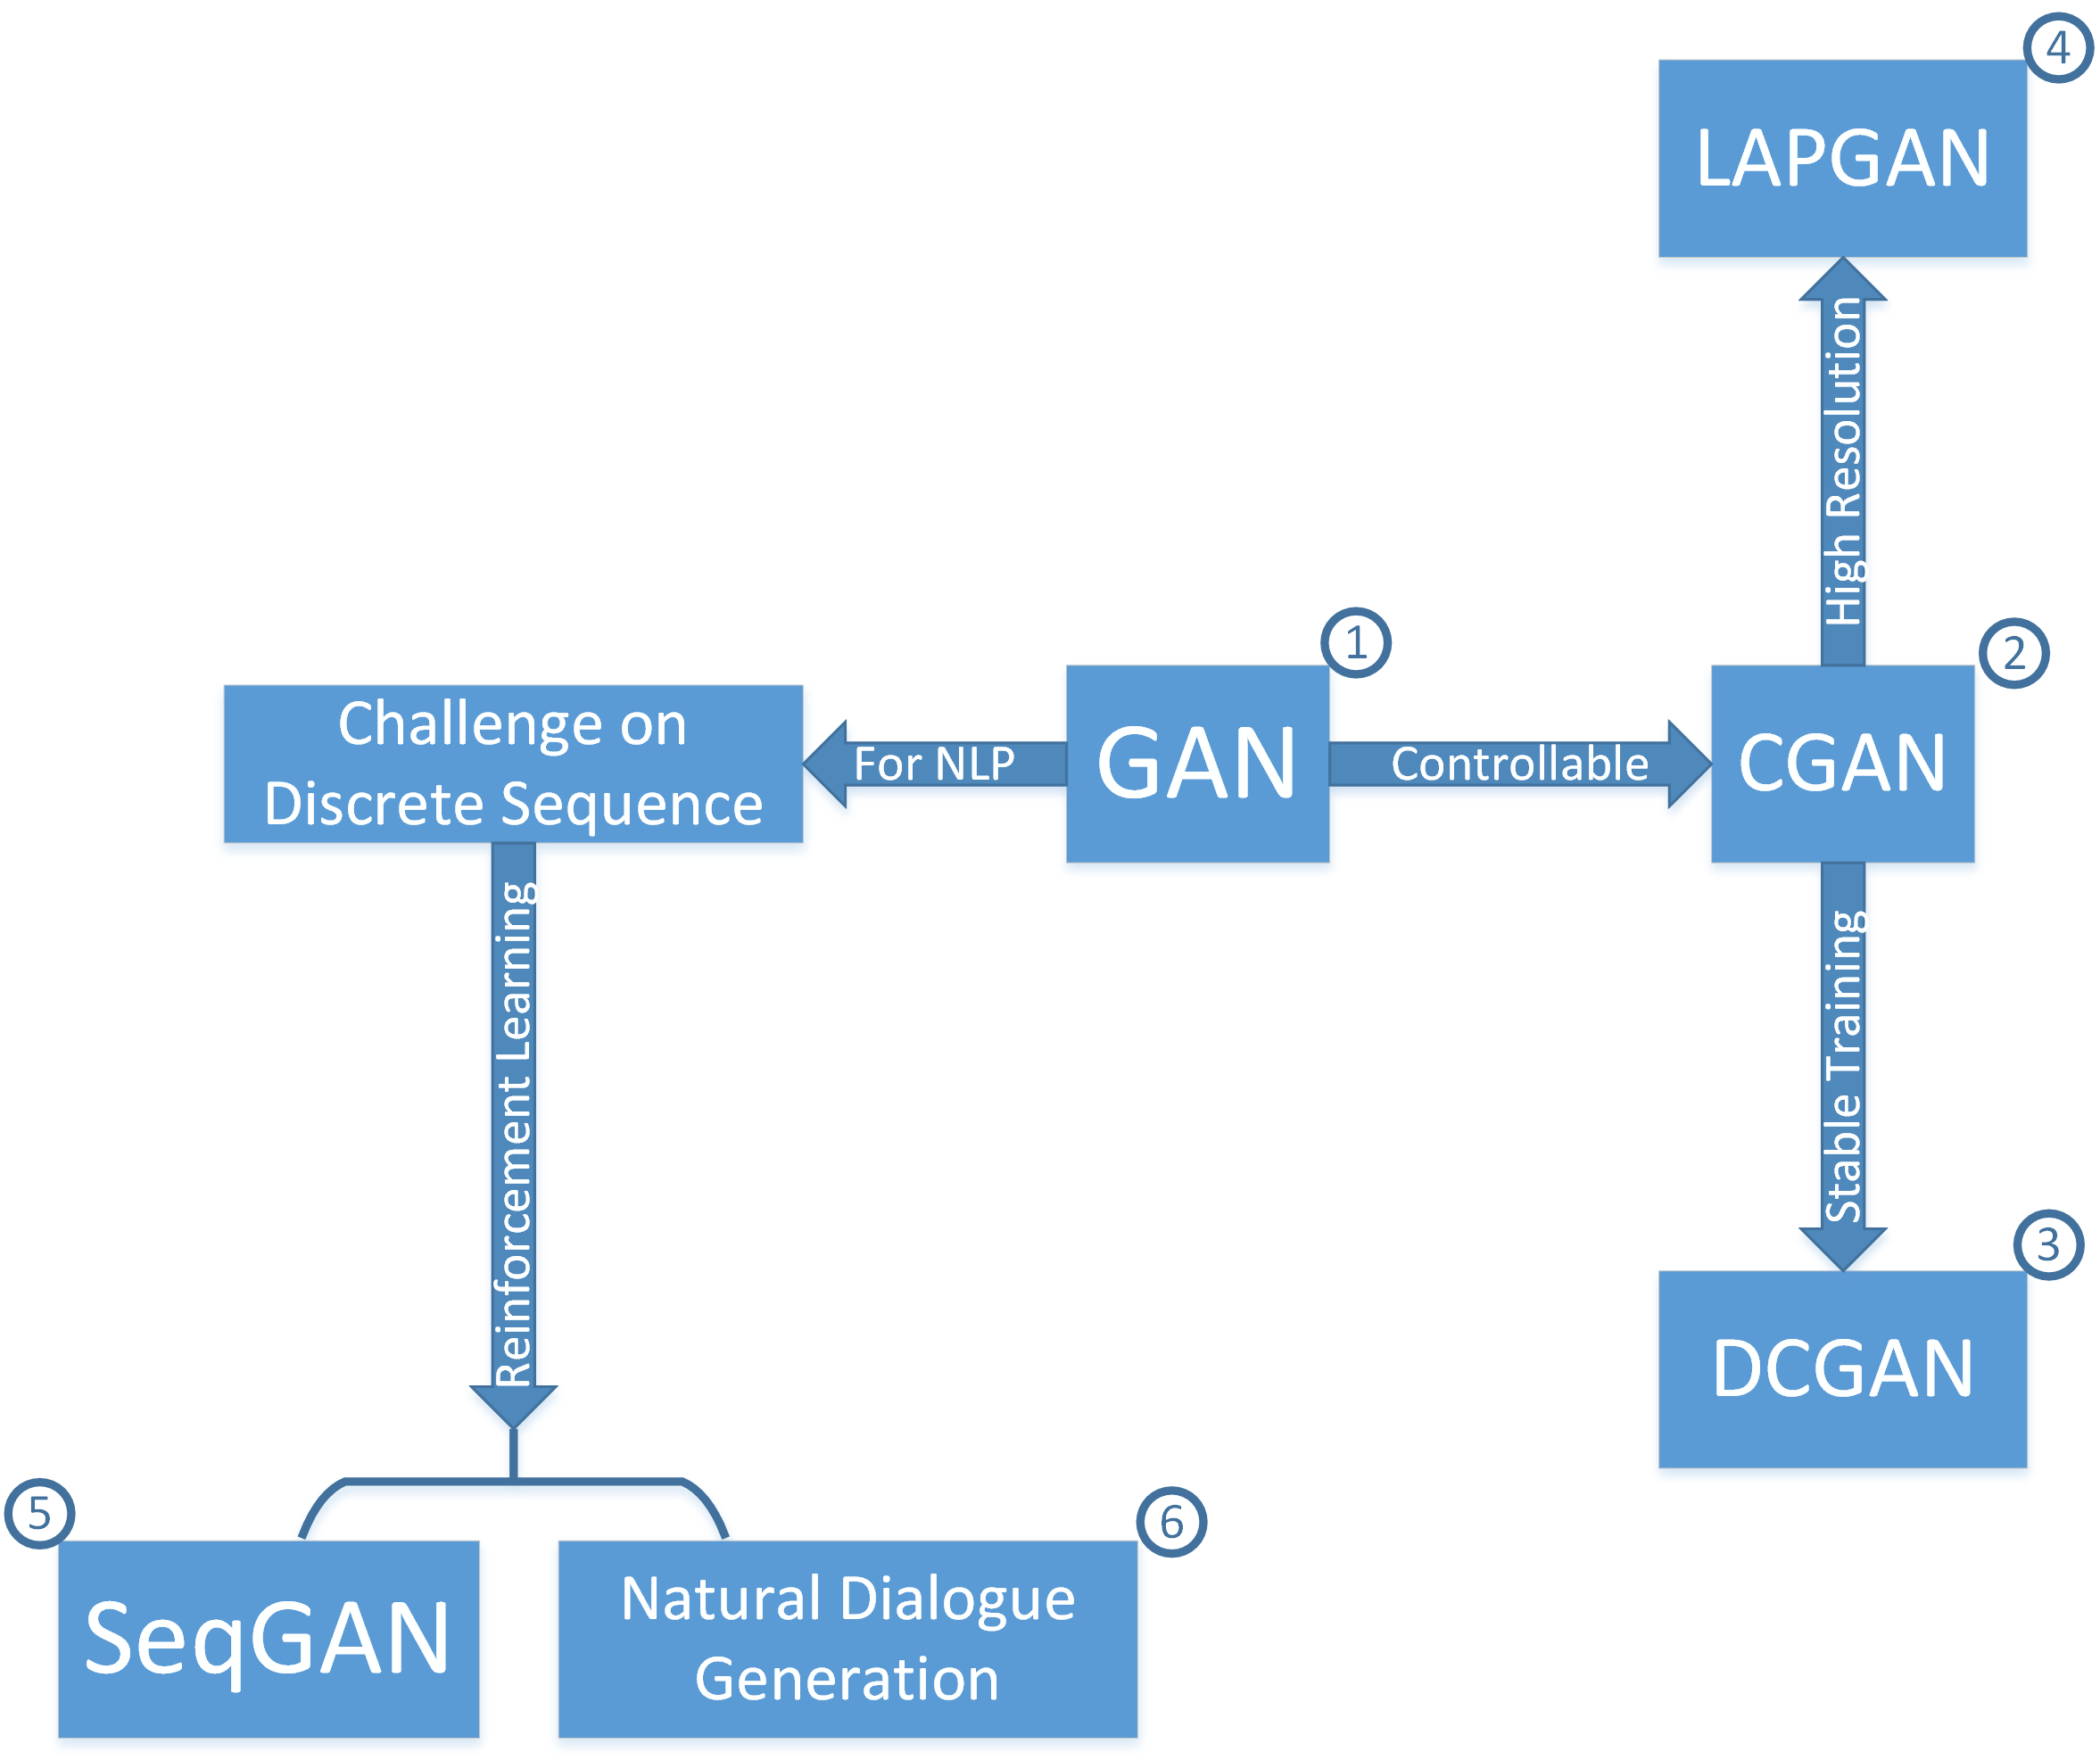
\includegraphics[width=25em]{figures/outline.png}
		\end{figure}
	\end{frame}

	\part{Background: Generative Model and Discriminative Model}
	\subtitlepage{Background Information}{Generative Model and Discriminative Model}{}
	\begin{frame}{Generative Model and Discriminative Model}
		What is generative model?
		\begin{itemize}
			\item Modelling the generation distribution of data.
			\item Done by modelling a joint probability distribution $p(x, y)$.
		\end{itemize}
		What is discriminative model?
		\begin{itemize}
			\item Modelling the dependence of an unobserved variable $y$ on an observed variable $x$.
			\item Done by modelling the conditional probability distribution $p(y|x)$.
			\item For tasks such as classification and regression that do not require the joint distribution, discriminative models can yield superior performance.
		\end{itemize}
		
		\textbf{generative models modelling the data, discriminative models modelling the difference between data}.
	\end{frame}

	\begin{frame}{Generative Model and Discriminative Model}
		Why we need generative model?
		\begin{itemize}
			\item We can get a discriminative model via a generative model by $p(y|x)=\frac{p(x, y)}{p(x)}$, the other way not. 
			\item We can \textbf{sample new data} from generative model whereas discriminative model cannot. (AMAZING!)
		\end{itemize}
		Is is easy to get a generative model?
		\begin{itemize}
			\item It is hard to estimate an probabilistic model.
			\item We need enough observed data + robust model.
		\end{itemize}
		How can we get a generative model?
		\begin{itemize}
			\item Gaussian mixture model and other types (GMM)
			\item Hidden Markov Model (HMM)
			\item Latent Dirichlet Allocation(LDA)
			\item Restricted Boltzmann Machine (RBM)
			\item \textbf{Generative Adversarial Networks (GAN)}
		\end{itemize}
	\end{frame}

	\part{GAN}
	\subtitlepage{}{Generative Adversarial Nets}{Ian J. Goodfellow, Jean Pouget-Abadie, Mehdi Mirza, Bing Xu, \\ David Warde-Farley, Sherjil Ozair, Aaron Courville, Yoshua Bengio. \\ NIPS 2014\\ arXiv: 1406.2661}
	
	\begin{frame}{Introduction of GAN}
		\begin{itemize}
			\item New framework for estimating generative models via an adversarial process.
			\item Train two models simultaneously:
			\begin{itemize}
				\item A generative model $G$ that captures the data distribution.
				\item A discriminative model $D$ that estimates the probability that a sample came from the training data rather than $G$.
			\end{itemize}
			\item A minimax two-player zero-sum game.
			\item Unique solution exists (ensuring convergence): $G$ recovering the training data distribution; $D=\frac{1}{2}$ everywhere.
		\end{itemize}
	\end{frame}

	\begin{frame}{Introduction of GAN}
		\begin{itemize}
			\item The purpose of generative model is to learn data distribution $p_g$.
			\item We have a noise variable $p_z(z)$ first, and sample a $z\sim p_z(z)$.
			\item Synthesized data $\hat{x}=G(z;\theta_g)$. $\theta_g$ is the parameter of the generative model.
			\item If the $\theta_g$ is well trained, we will get a generative model $p_g\approx p_{\text{data}}$. ($p_g$ have learned the same mapping function as $p_{\text{data}}$)
			\item In this case, we can generate new "fake" data realistic enough to confuse human as well as the discriminator.
			\item AMAZING! Our model has learned the distribution of data and can generate new sample!
			\item For example: produce "reasonable" images.
		\end{itemize}
	\end{frame}

	\begin{frame}{Adversarial nets}
		\begin{figure}
			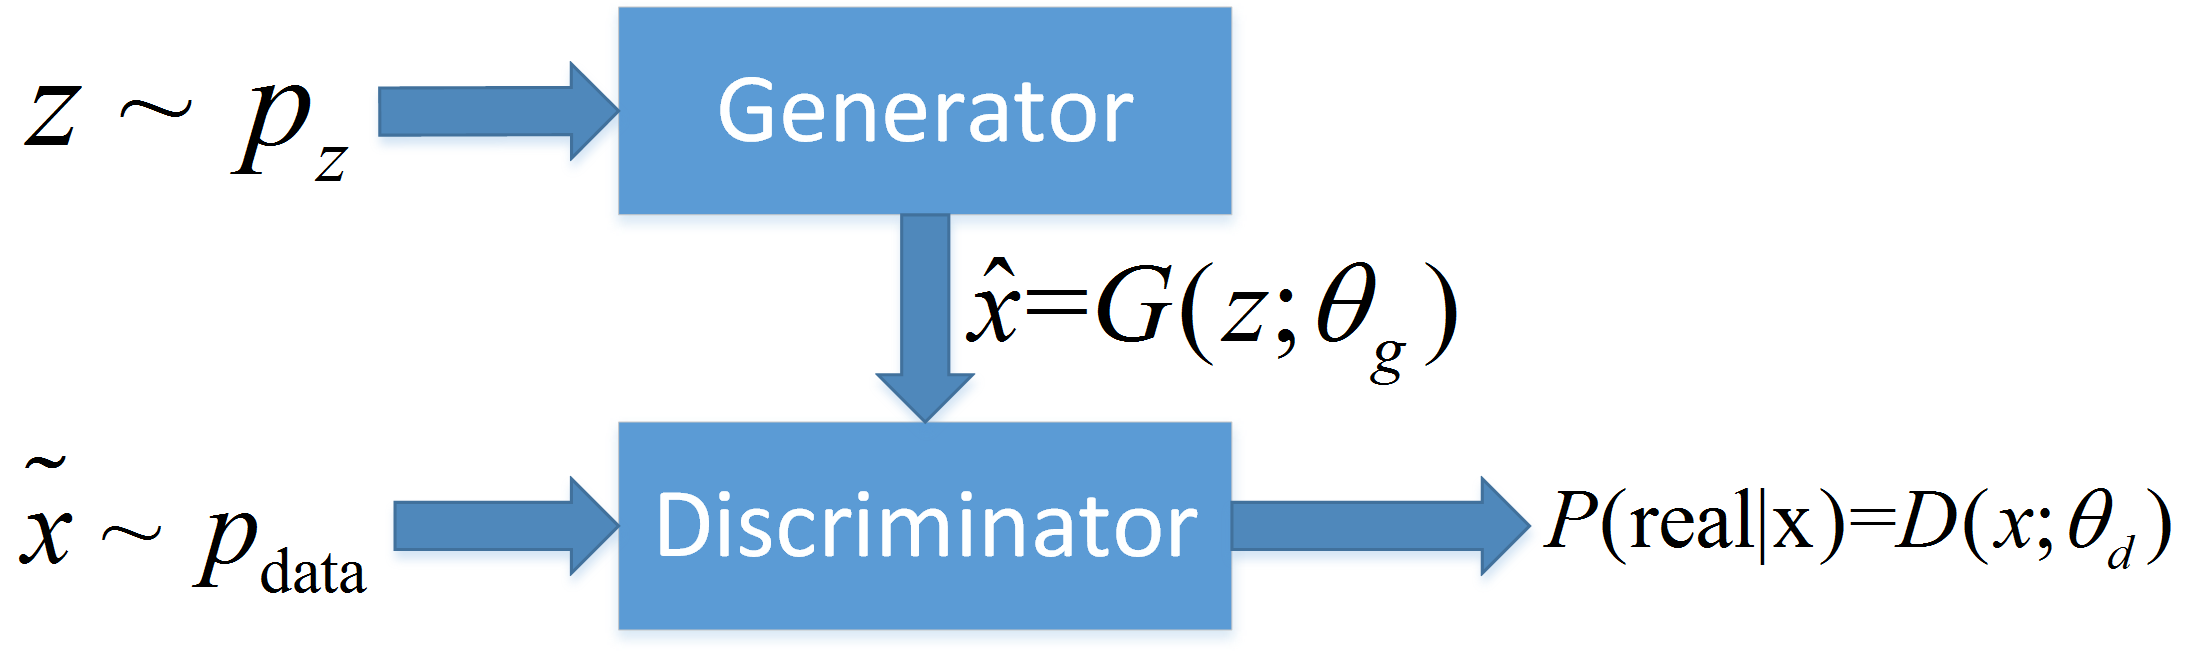
\includegraphics[width=25em]{figures/GAN-general-structure.png}
		\end{figure}
		We train $D$ to maximize the probability of assigning the correct label to both training examples and samples from $G$.
	
		We simultaneously train $G$ to minimize $\log(1-D(G(\bm{z})))$. In other words, $D$ and $G$ play the following two-player minimax game with value function $V(G,D)$:
		$$
		\mathop{\min}_{G}\mathop{\max}_{D}V(D,G)=\mathbb{E}_{\bm{x}\sim p_{\text{data}}}\left[\log D(\bm{x})\right]+\mathbb{E}_{\bm{z}\sim p_z(\bm{z})}\left[\log(1-D(G(\bm{z})))\right].
		$$
		
	\end{frame}

	\begin{frame}{Adversarial nets}
		Why we need the discriminator? Why can't we define the loss function as the MSE of the real image and the image produced by the generator directly?
		\begin{figure}
			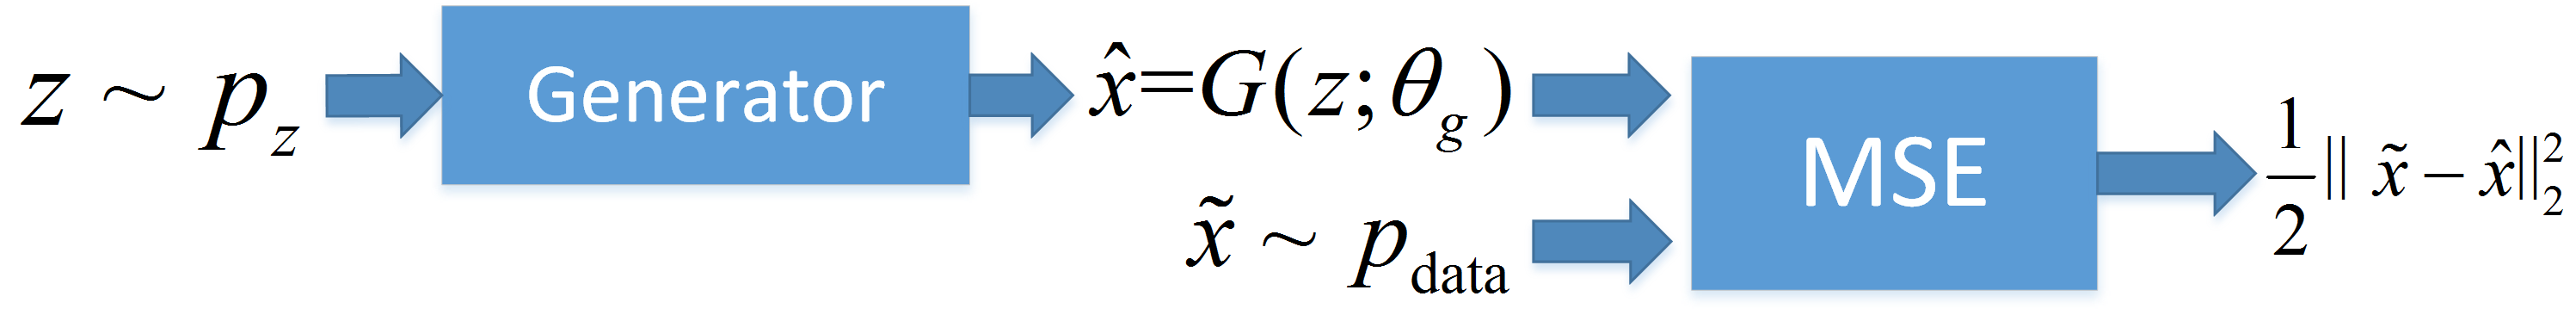
\includegraphics[width=25em]{figures/GAN-hypothesis-structure.png}
		\end{figure}
		If we only have the generator, this model can be regarded as an unsupervised learning problem. But if we want the output image of the generator as similar as possible to the training sample, the generator will finally remember all the training data and it will not be able to produce any "new" images.
	\end{frame}

	\begin{frame}[t]{Adversarial nets}
		Here is a less formal, more pedagogical explanation of the approach:
		\begin{figure}
			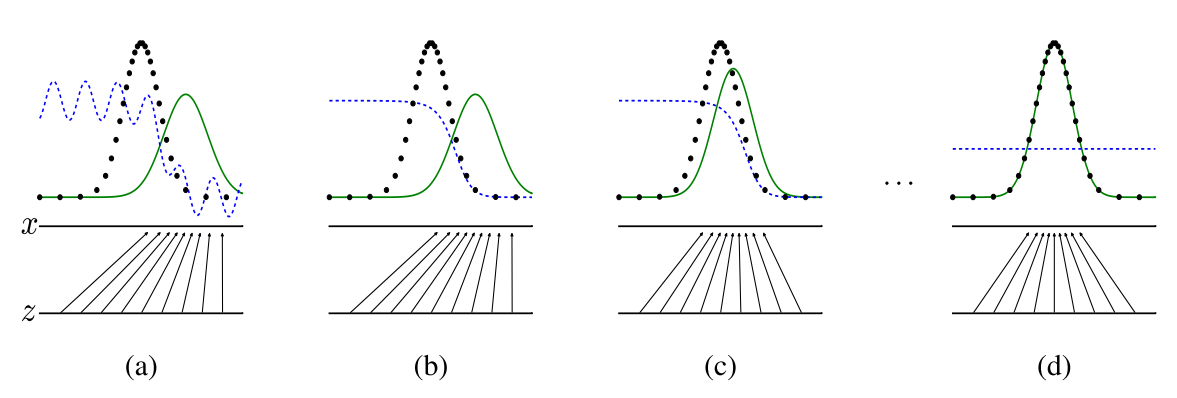
\includegraphics[width=25em]{figures/GAN-pedagogical-explanation.png}
		\end{figure}
		Generative adversarial nets are trained by simultaneously updating the \textbf{d}iscriminative distribution (D, blue, dashed line) so that it discriminates between samples from the data generating distribution (black, dotted line) $p_g$ from those of the \textbf{g}enerative distribution $p_g(G)$ (green, solid line). 
	\end{frame}
	
	\begin{frame}[t]{Adversarial nets}
		Here is a less formal, more pedagogical explanation of the approach:
		\begin{figure}
			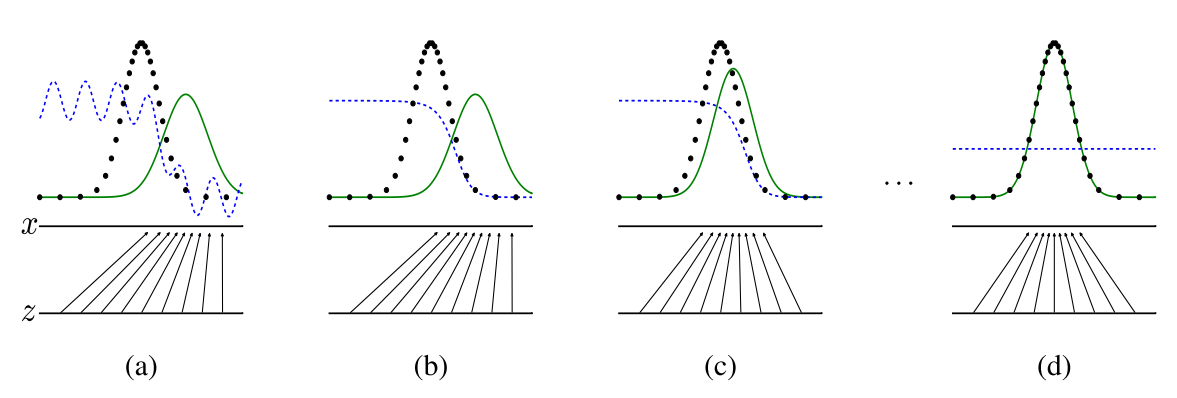
\includegraphics[width=25em]{figures/GAN-pedagogical-explanation.png}
		\end{figure}
	 	The lower horizontal line is the domain from which $\bm{z}$ is sampled, in this case uniformly. The horizontal line above is part of the domain of $\bm{x}$. The upward arrows show how the mapping $\bm{x}=G(\bm{z})$ imposes the non-uniform distribution $p_g$ on transformed samples.
	\end{frame}

	\begin{frame}[t]{Adversarial nets}
		Here is a less formal, more pedagogical explanation of the approach:
		\begin{figure}
			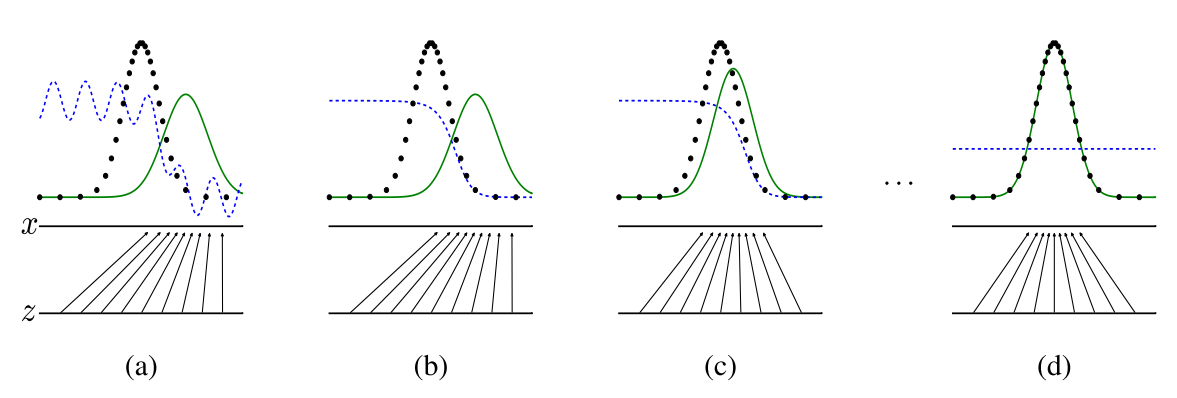
\includegraphics[width=25em]{figures/GAN-pedagogical-explanation.png}
		\end{figure}
		(a) Consider an adversarial pair near convergence: $p_g$ is similar to $p_{\text{data}}$ and $D$ is a partially accurate classifier.
		
		(b) In the inner loop of the algorithm $D$ is trained to discriminate samples from data, converging to $D^*(\bm{x})=\frac{p_{\text{data}}(\bm{x})}{p_{\text{data}}(\bm{x})+p_g(\bm{x})}$
	\end{frame}

	\begin{frame}[t]{Adversarial nets}
		Here is a less formal, more pedagogical explanation of the approach:
		\begin{figure}
			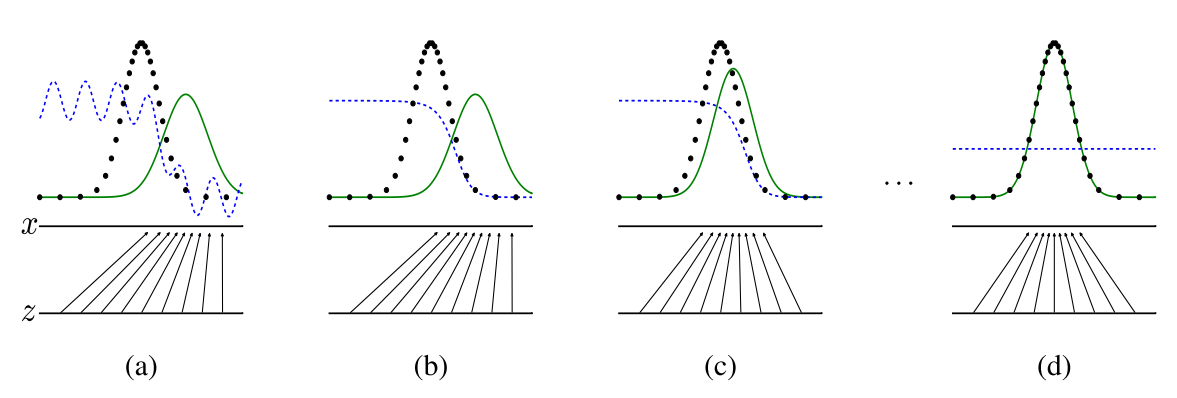
\includegraphics[width=25em]{figures/GAN-pedagogical-explanation.png}
		\end{figure}
		(c) After an update to $G$, gradient of $D$ has guided $G(\bm{z})$ to flow to regions that are more likely to be classified as data.
		
		(d) After several steps of training, if $G$ and $D$ have enough capacity, they will reach a point at which both cannot improve because $p_g=p_{\text{data}}$.
	\end{frame}

	\begin{frame}[t]{Adversarial nets}
		Here is a less formal, more pedagogical explanation of the approach:
		\begin{figure}
			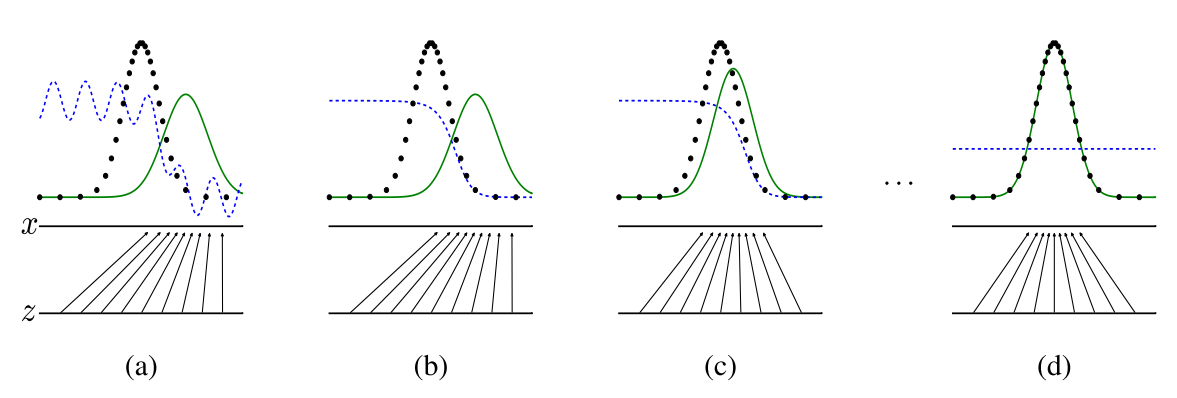
\includegraphics[width=25em]{figures/GAN-pedagogical-explanation.png}
		\end{figure}
		The discriminator is unable to differentiate between the two distributions. i.g. $D(\bm{x})=\frac{1}{2}$
	\end{frame}

	\begin{frame}{Adversarial nets}
	
		\begin{itemize}
			\item There are several trifles we need to deal with. The first is insufficient gradient in the early learning.
			
			\item Let's take a look at the loss function again:
			$$
			\mathop{\min}_{G}\mathop{\max}_{D}V(D,G)=\mathbb{E}_{\bm{x}\sim p_{\text{data}}}\left[\log D(\bm{x})\right]+\mathbb{E}_{\bm{z}\sim p_z(\bm{z})}\left[\log(1-D(G(\bm{z})))\right].
			$$
			\item In practice, this equation may not provide sufficient gradient for $G$ to learn well.
			\item Early in learning, when $G$ is poor, $D$ can reject samples with high confidence because they are clearly different from the training data.
			\item In this case, $\log(1-D(G(z)))$ saturates.
			\item Rather than training $G$ to minimize $\log(1-D(G(\bm{z})))$ we can train $G$ to maximize $\log D(G(\bm{z}))$.
			\begin{eqnarray*}
			&&\mathop{\max}_{D}\mathbb{E}_{\bm{x}\sim p_{\text{data}}}\left[\log D(\bm{x})\right]+\mathbb{E}_{\bm{z}\sim p_z(\bm{z})}\left[\log(1-D(G(\bm{z})))\right] \\
			&&\mathop{\max}_{G}\mathbb{E}_{\bm{z}\sim p_{\text{z}}}\left[\log D(G(\bm{z}))\right]
			\end{eqnarray*}
		\end{itemize}
	\end{frame}

	\begin{frame}{Adversarial nets}
		\begin{itemize}
			\item The second trifle is that we need to prevent the overfit of $G$.
			\item We should conduct the iterative training: optimize the discriminator $k$ times and then train the generator once. 
		\end{itemize}
		\begin{algorithm}[H]
			\algsetup{linenosize=\tiny}
			\scriptsize
			%\tiny
			\caption{\scriptsize Minibatch stochastic gradient descent training of generative adversarial nets.}
			\label{alg:train-gan}
			\begin{algorithmic}
				\FOR{number of training iterations}
					\FOR{$k$ steps}
						\STATE Sample minibatch of $m$ noise samples $\{z^{(1)},\dots,z^{(m)}\}$ from noise prior $p_g(\bm{z})$
						\STATE Sample minibatch of $m$ examples ${x^{(1)},\dots,x^{(m)}}$ from data generating distribution $p_{\text{data}}(\bm{x})$
						\STATE Update the discriminator by ascending its stochastic gradient:
							\vspace{-1em}
							$$
							\nabla_{\theta_{d}}\frac{1}{m}\sum^m_{i=1}\left[\log D\left(\bm{x}^{(i)}\right)+\log\left(1-D\left(G\left(\bm{z}^{(i)}\right)\right)\right)\right]
							$$
							\vspace{-1em}
					\ENDFOR
					\STATE Sample minibatch of $m$ noise samples ${z^{(1)},\dots,z^{(m)}}$ from noise prior $p_g(\bm{z})$.
					\STATE Update the generator by descending its stochastic gradient:
						\vspace{-1em}
						$$
						\nabla_{\theta_{d}}\frac{1}{m}\sum_{i=1}^{m}\log\left(1-D\left(G\left(\bm{z}^{(i)}\right)\right)\right)
						$$
						\vspace{-1em}
				\ENDFOR
			\end{algorithmic}
		\end{algorithm}
	\end{frame}

	\begin{frame}{Experiments}
		\begin{itemize}
			\item MNIST.
			\item Toronto Face Database(TFD).
			\item CIFAR-10.
		\end{itemize}
		\begin{figure}
			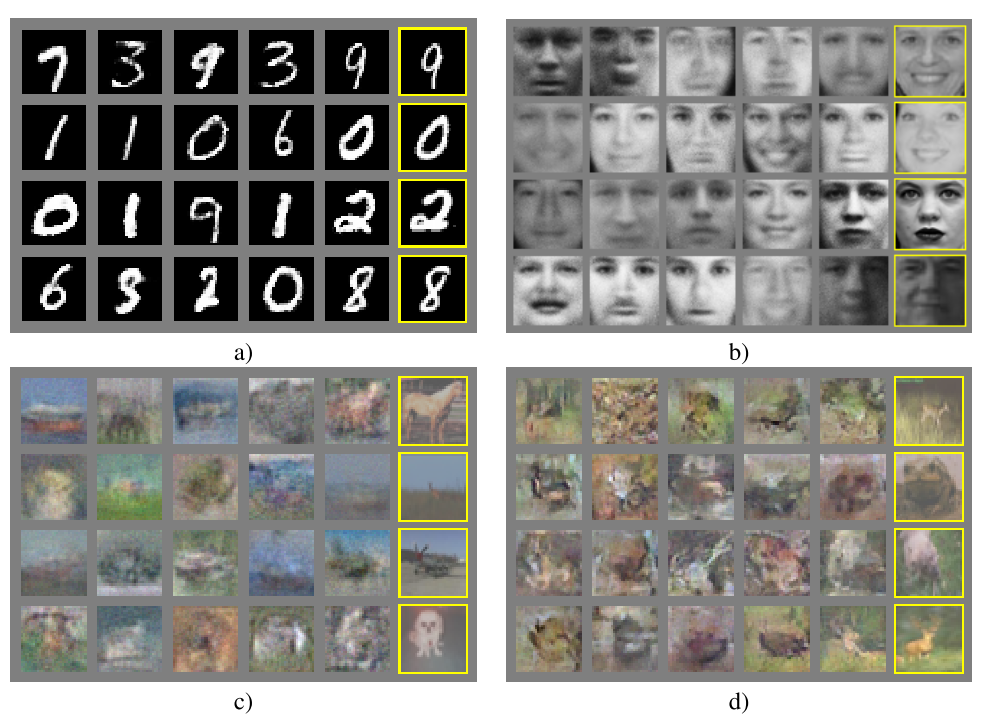
\includegraphics[width=25em]{figures/GAN-experiment-demo-pic.png}
		\end{figure}
	\end{frame}

	\part{CGAN}
	\begin{frame}{Outline}
		\begin{figure}
			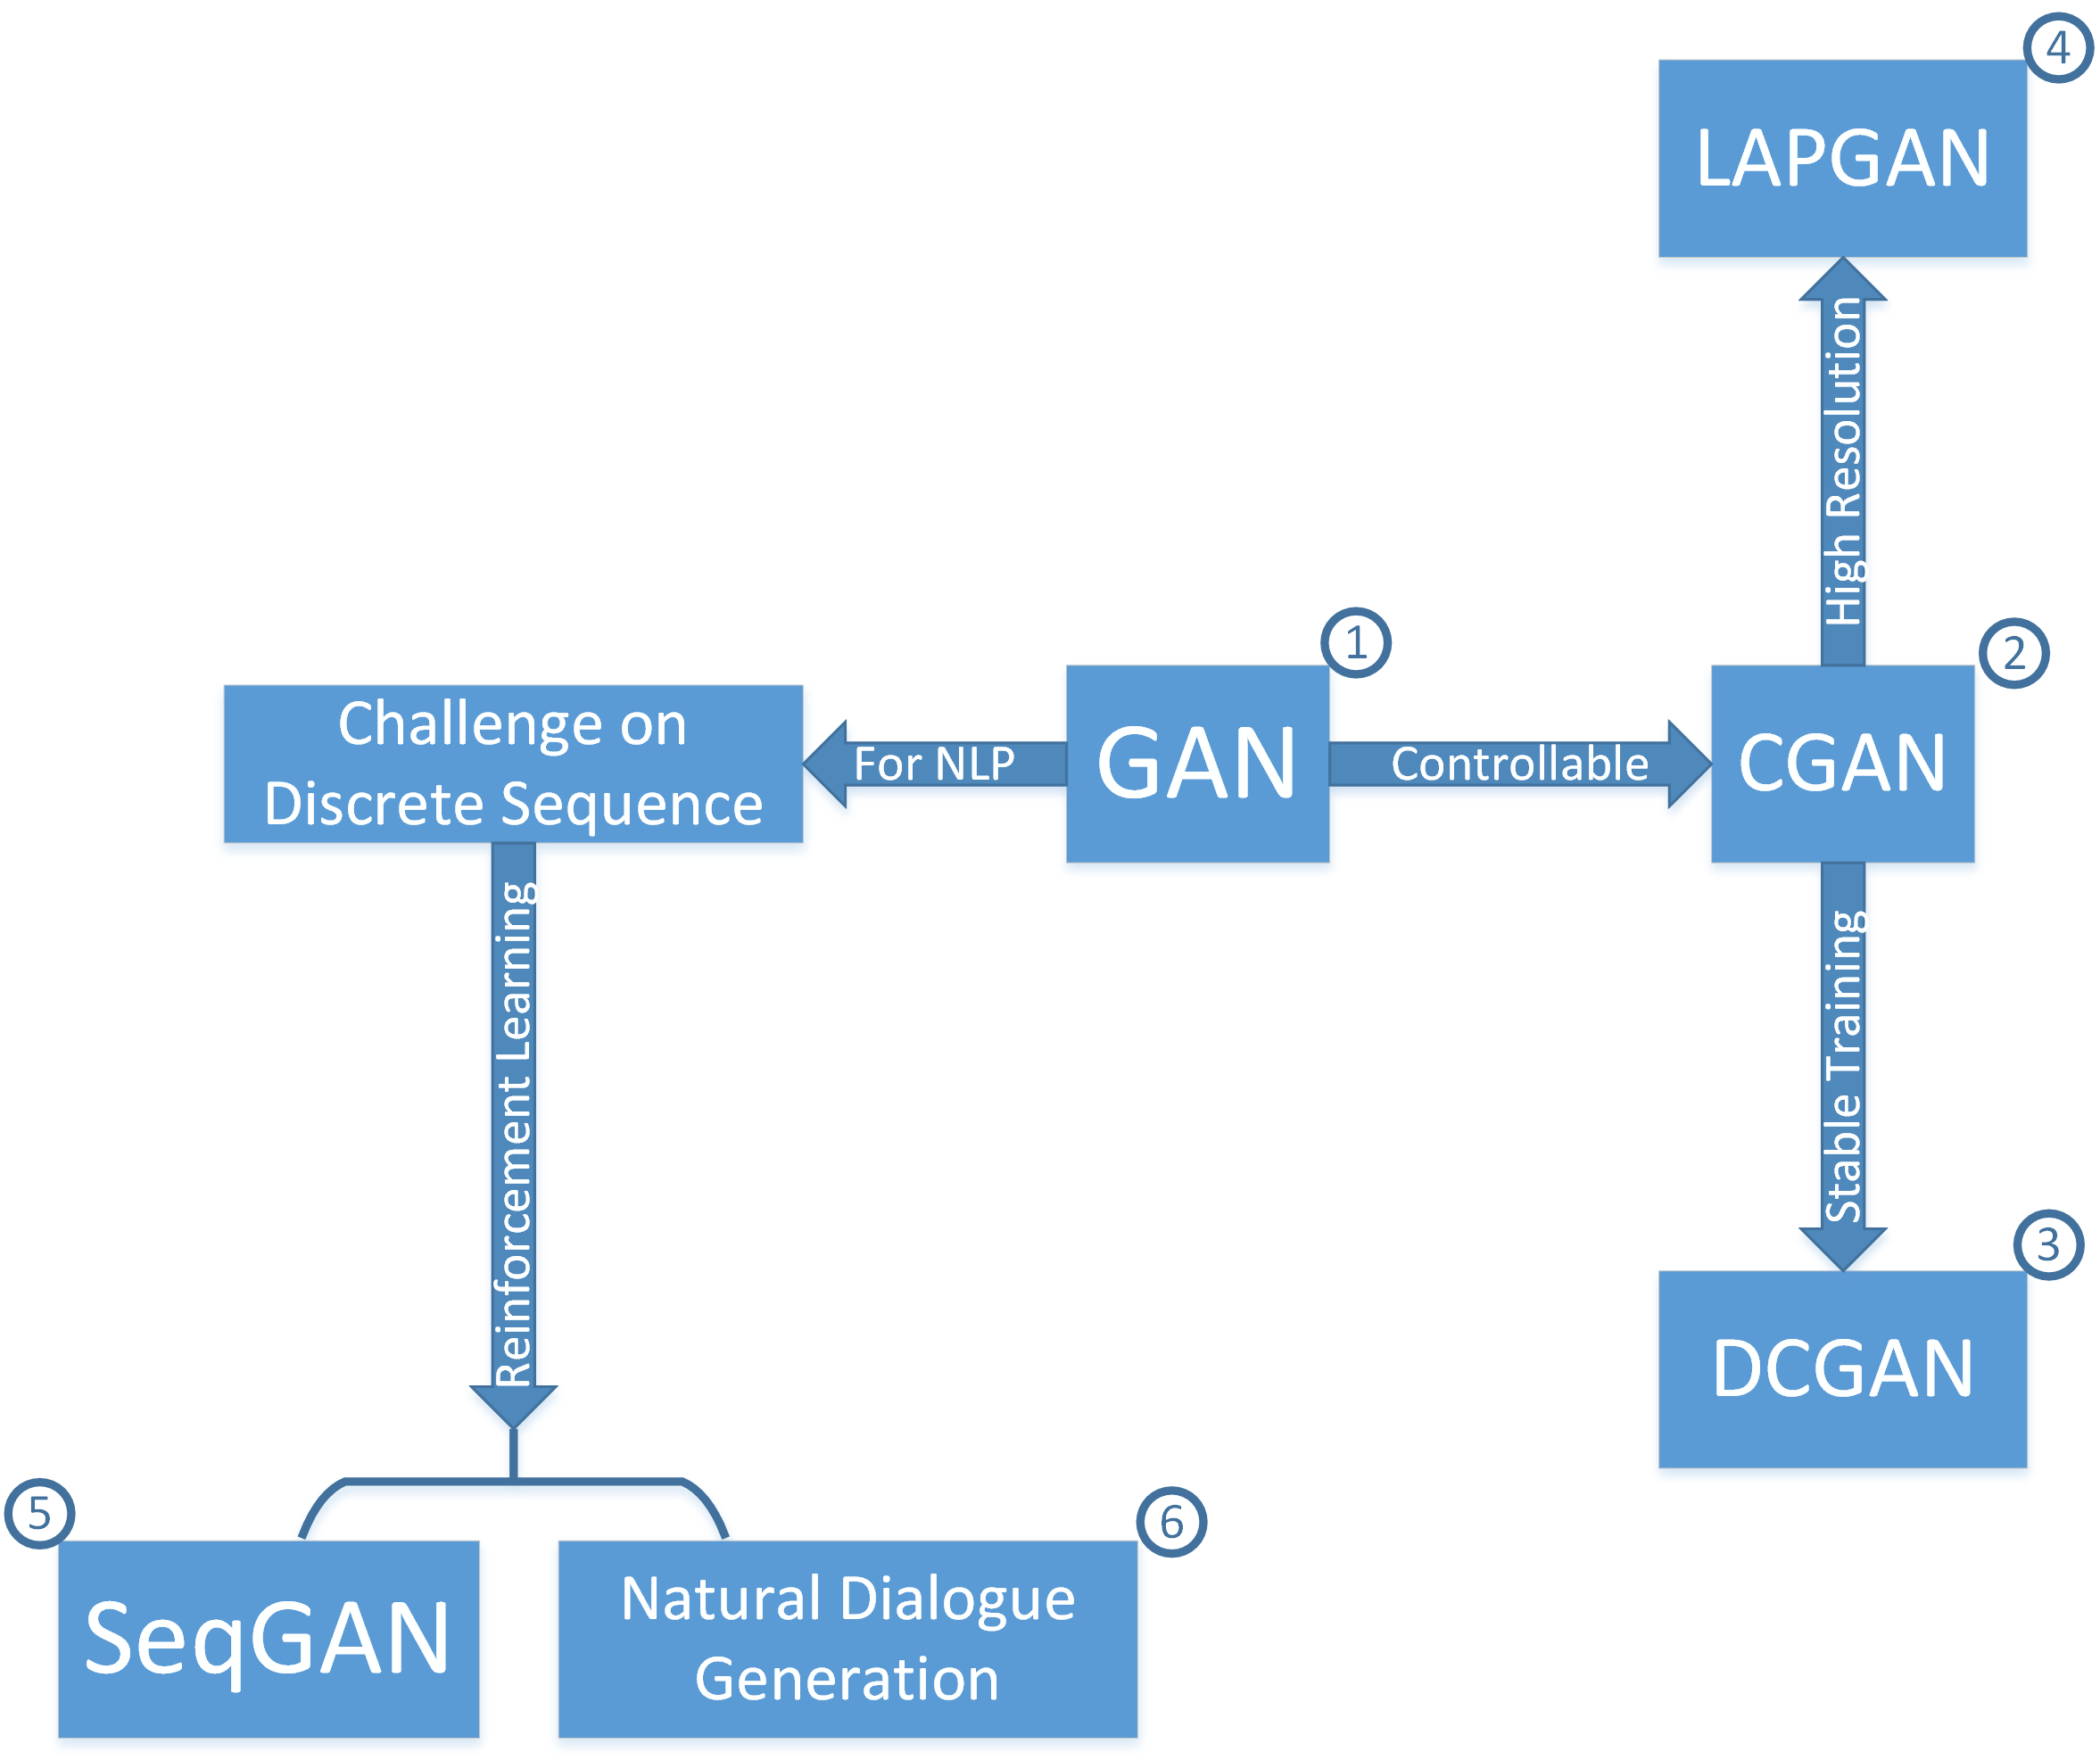
\includegraphics[width=25em]{figures/outline.png}
		\end{figure}
	\end{frame}
	\subtitlepage{}{Conditional Generative Adversarial Nets}{Mehdi Mirza, Simon Osindero\\arXiv: 1411.1784}
	
	\begin{frame}{Introduction}
		\begin{itemize}
			\item Generative adversarial nets were recently introduced as an alternative framework for training generative models.
			\item In an unconditioned generative model, there is no control on models of the data being generated.
			\item By conditioning the model on additional information it is possible to direct the data generating process.
			\item Such conditioning could be based on class labels, on some part of data, or even on data from different modality.
		\end{itemize}
	\end{frame}

	\begin{frame}{Introduction}
		\begin{itemize}
			\item Optimization object of unconditioned generative model:
			$$
			\mathop{\min}_{G}\mathop{\max}_{D}V(D,G)=\mathbb{E}_{\bm{x}\sim p_{\text{data}}}\left[\log D(\bm{x})\right]+\mathbb{E}_{\bm{z}\sim p_z(\bm{z})}\left[\log(1-D(G(\bm{z})))\right].
			$$
			\item Optimization object of conditioned generative model:
			$$
			\mathop{\min}_{G}\mathop{\max}_{D}V(D,G)=\mathbb{E}_{\bm{x}\sim p_{\text{data}}}\left[\log D(\bm{x}|\bm{y})\right]+\mathbb{E}_{\bm{z}\sim p_z(\bm{z})}\left[\log(1-D(G(\bm{z}|\bm{y})|\bm{y}))\right].
			$$
		\end{itemize}
	\end{frame}

	\begin{frame}{Structure}
		\begin{figure}
			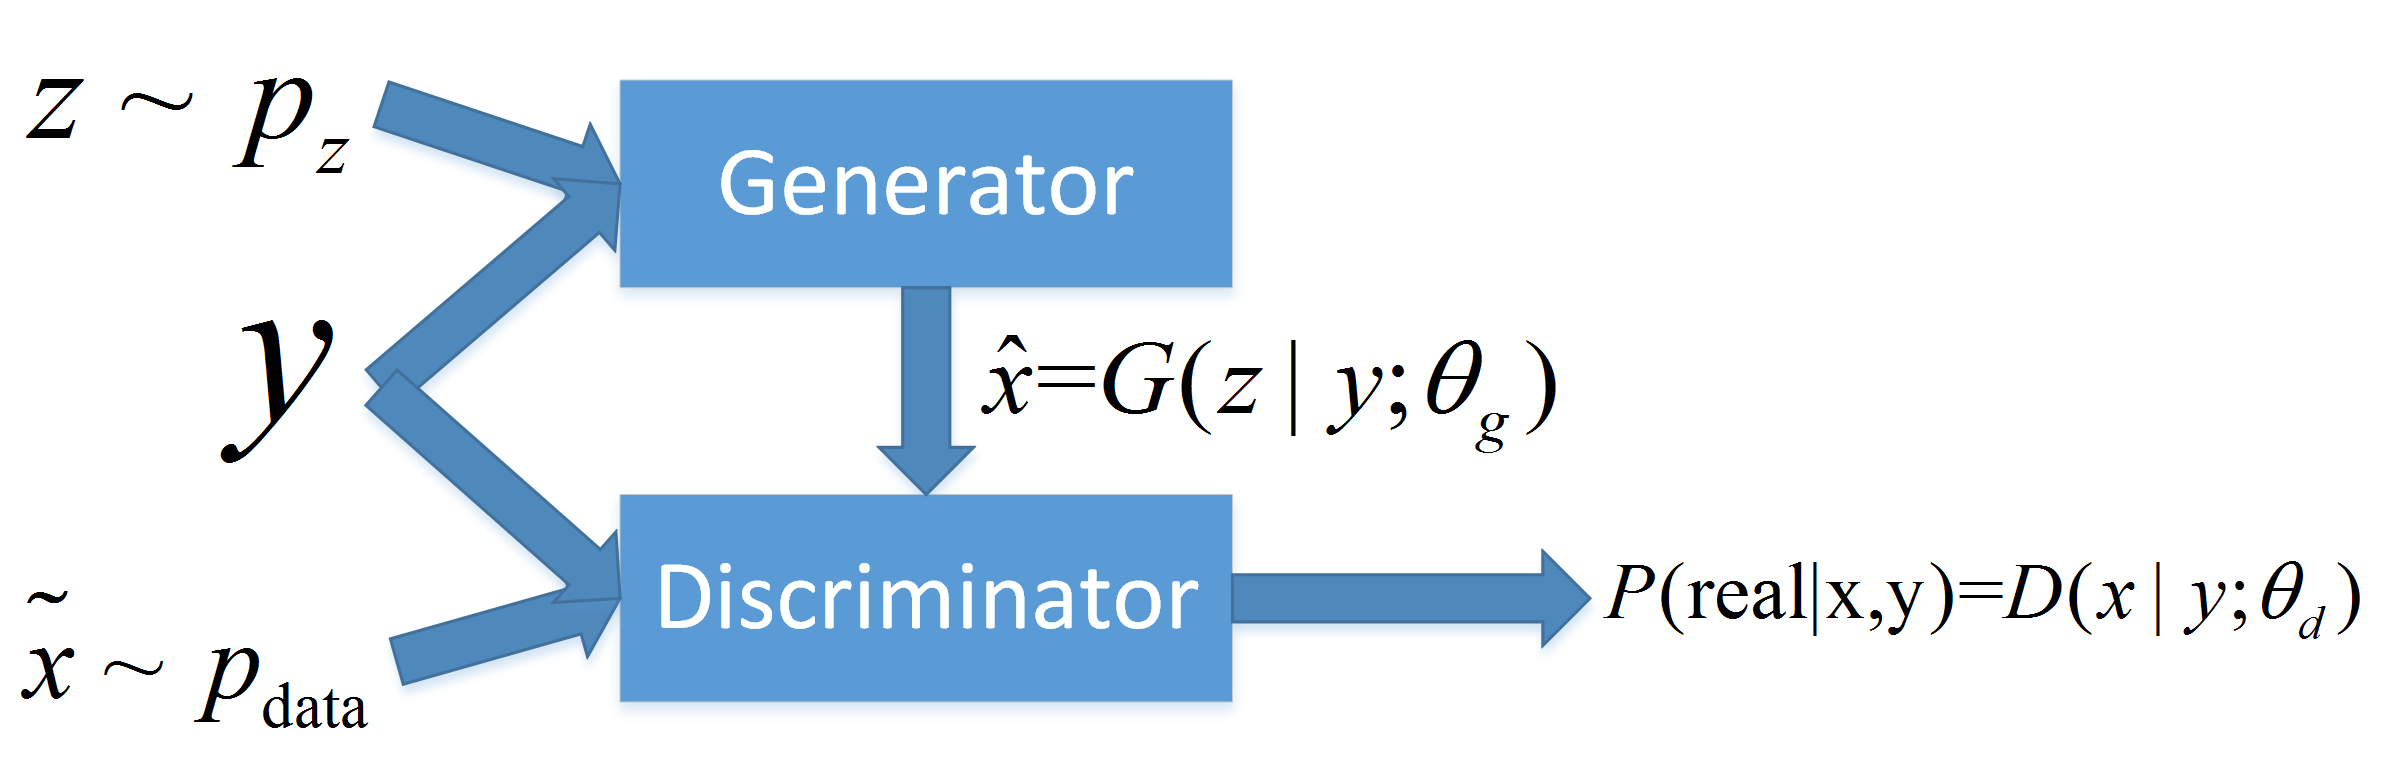
\includegraphics[width=20em]{figures/CGAN-general-structure.png}
		\end{figure}
		\begin{figure}
			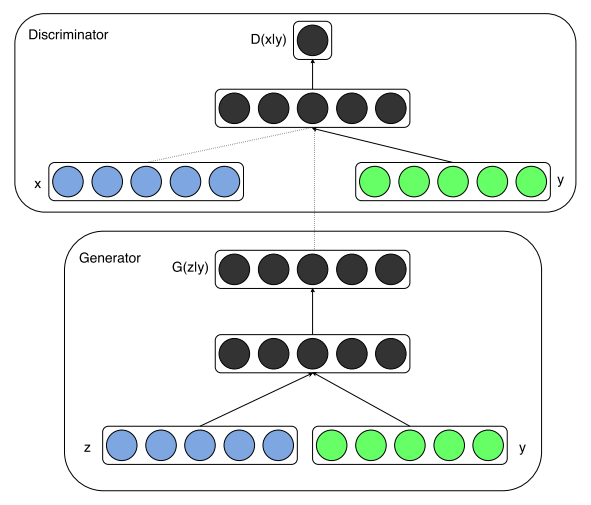
\includegraphics[width=15em]{figures/CGAN-origin-structure.png}
		\end{figure}
	\end{frame}

	\begin{frame}{Experiment}
		\begin{itemize}
			\item Experiment on MNIST
			\item $y$ is the 10 classes of digit represent in one-hot vector.
			\begin{figure}
				\caption{Generated MNIST digits, each row conditioned on one label}
				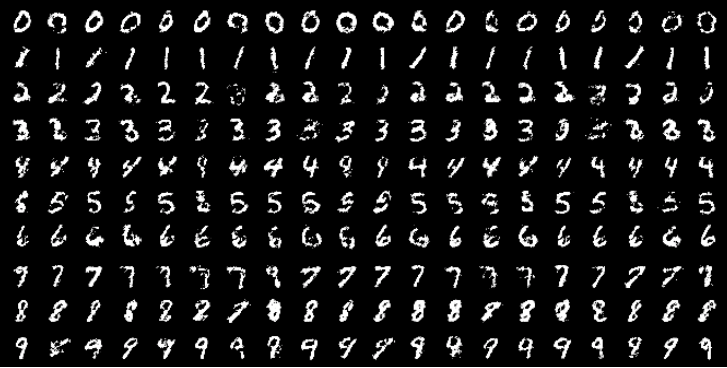
\includegraphics[width=25em]{figures/CGAN-experiment-mnist.png}
			\end{figure}
		\end{itemize}
	\end{frame}

	\begin{frame}{Experiment (Multi-modal)}
		\begin{itemize}
			\item Pretrained image feature extractor and skip-gram model for word representation.
			\item Trained a convolutional image feature extractor on full ImageNet dataset.
			\item Trained a skip-gram model for word representation: a $\mathrm{R}^{200}$ word vector on YFCC100M(Yahoo Flickr Creative Common 100M) dataset meta-data.
			\item Conducted experiment on MIR Flickr 25,000 dataset, extract the image and tags features using the convolution model and embedding model.
		\end{itemize}
	\end{frame}

	\begin{frame}{Experiment (Multi-modal)}
		\begin{figure}
			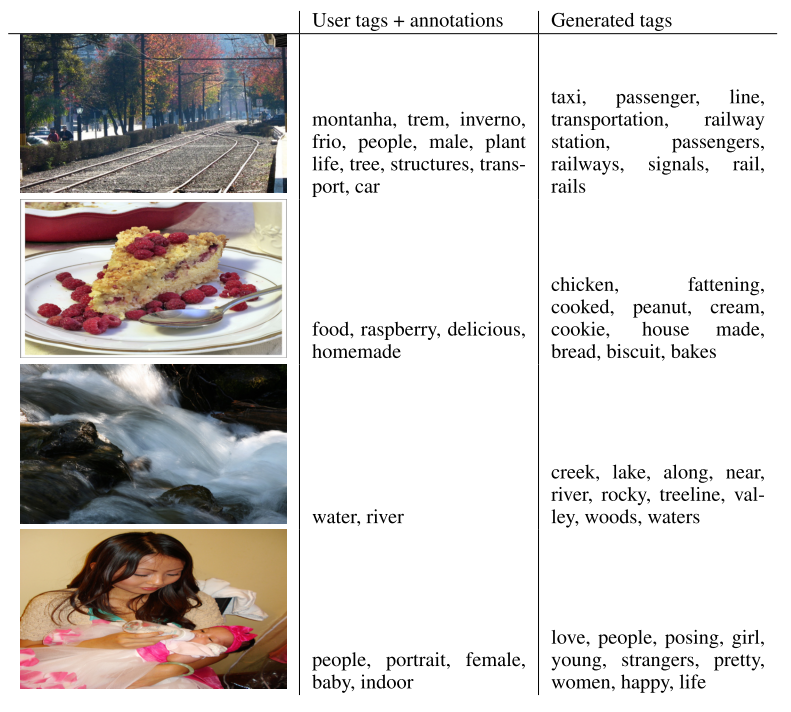
\includegraphics[width=25em]{figures/CGAN-experiment-multi-modal.png}
		\end{figure}
	\end{frame}
	
	\part{DCGAN}
	\begin{frame}{Outline}
		\begin{figure}
			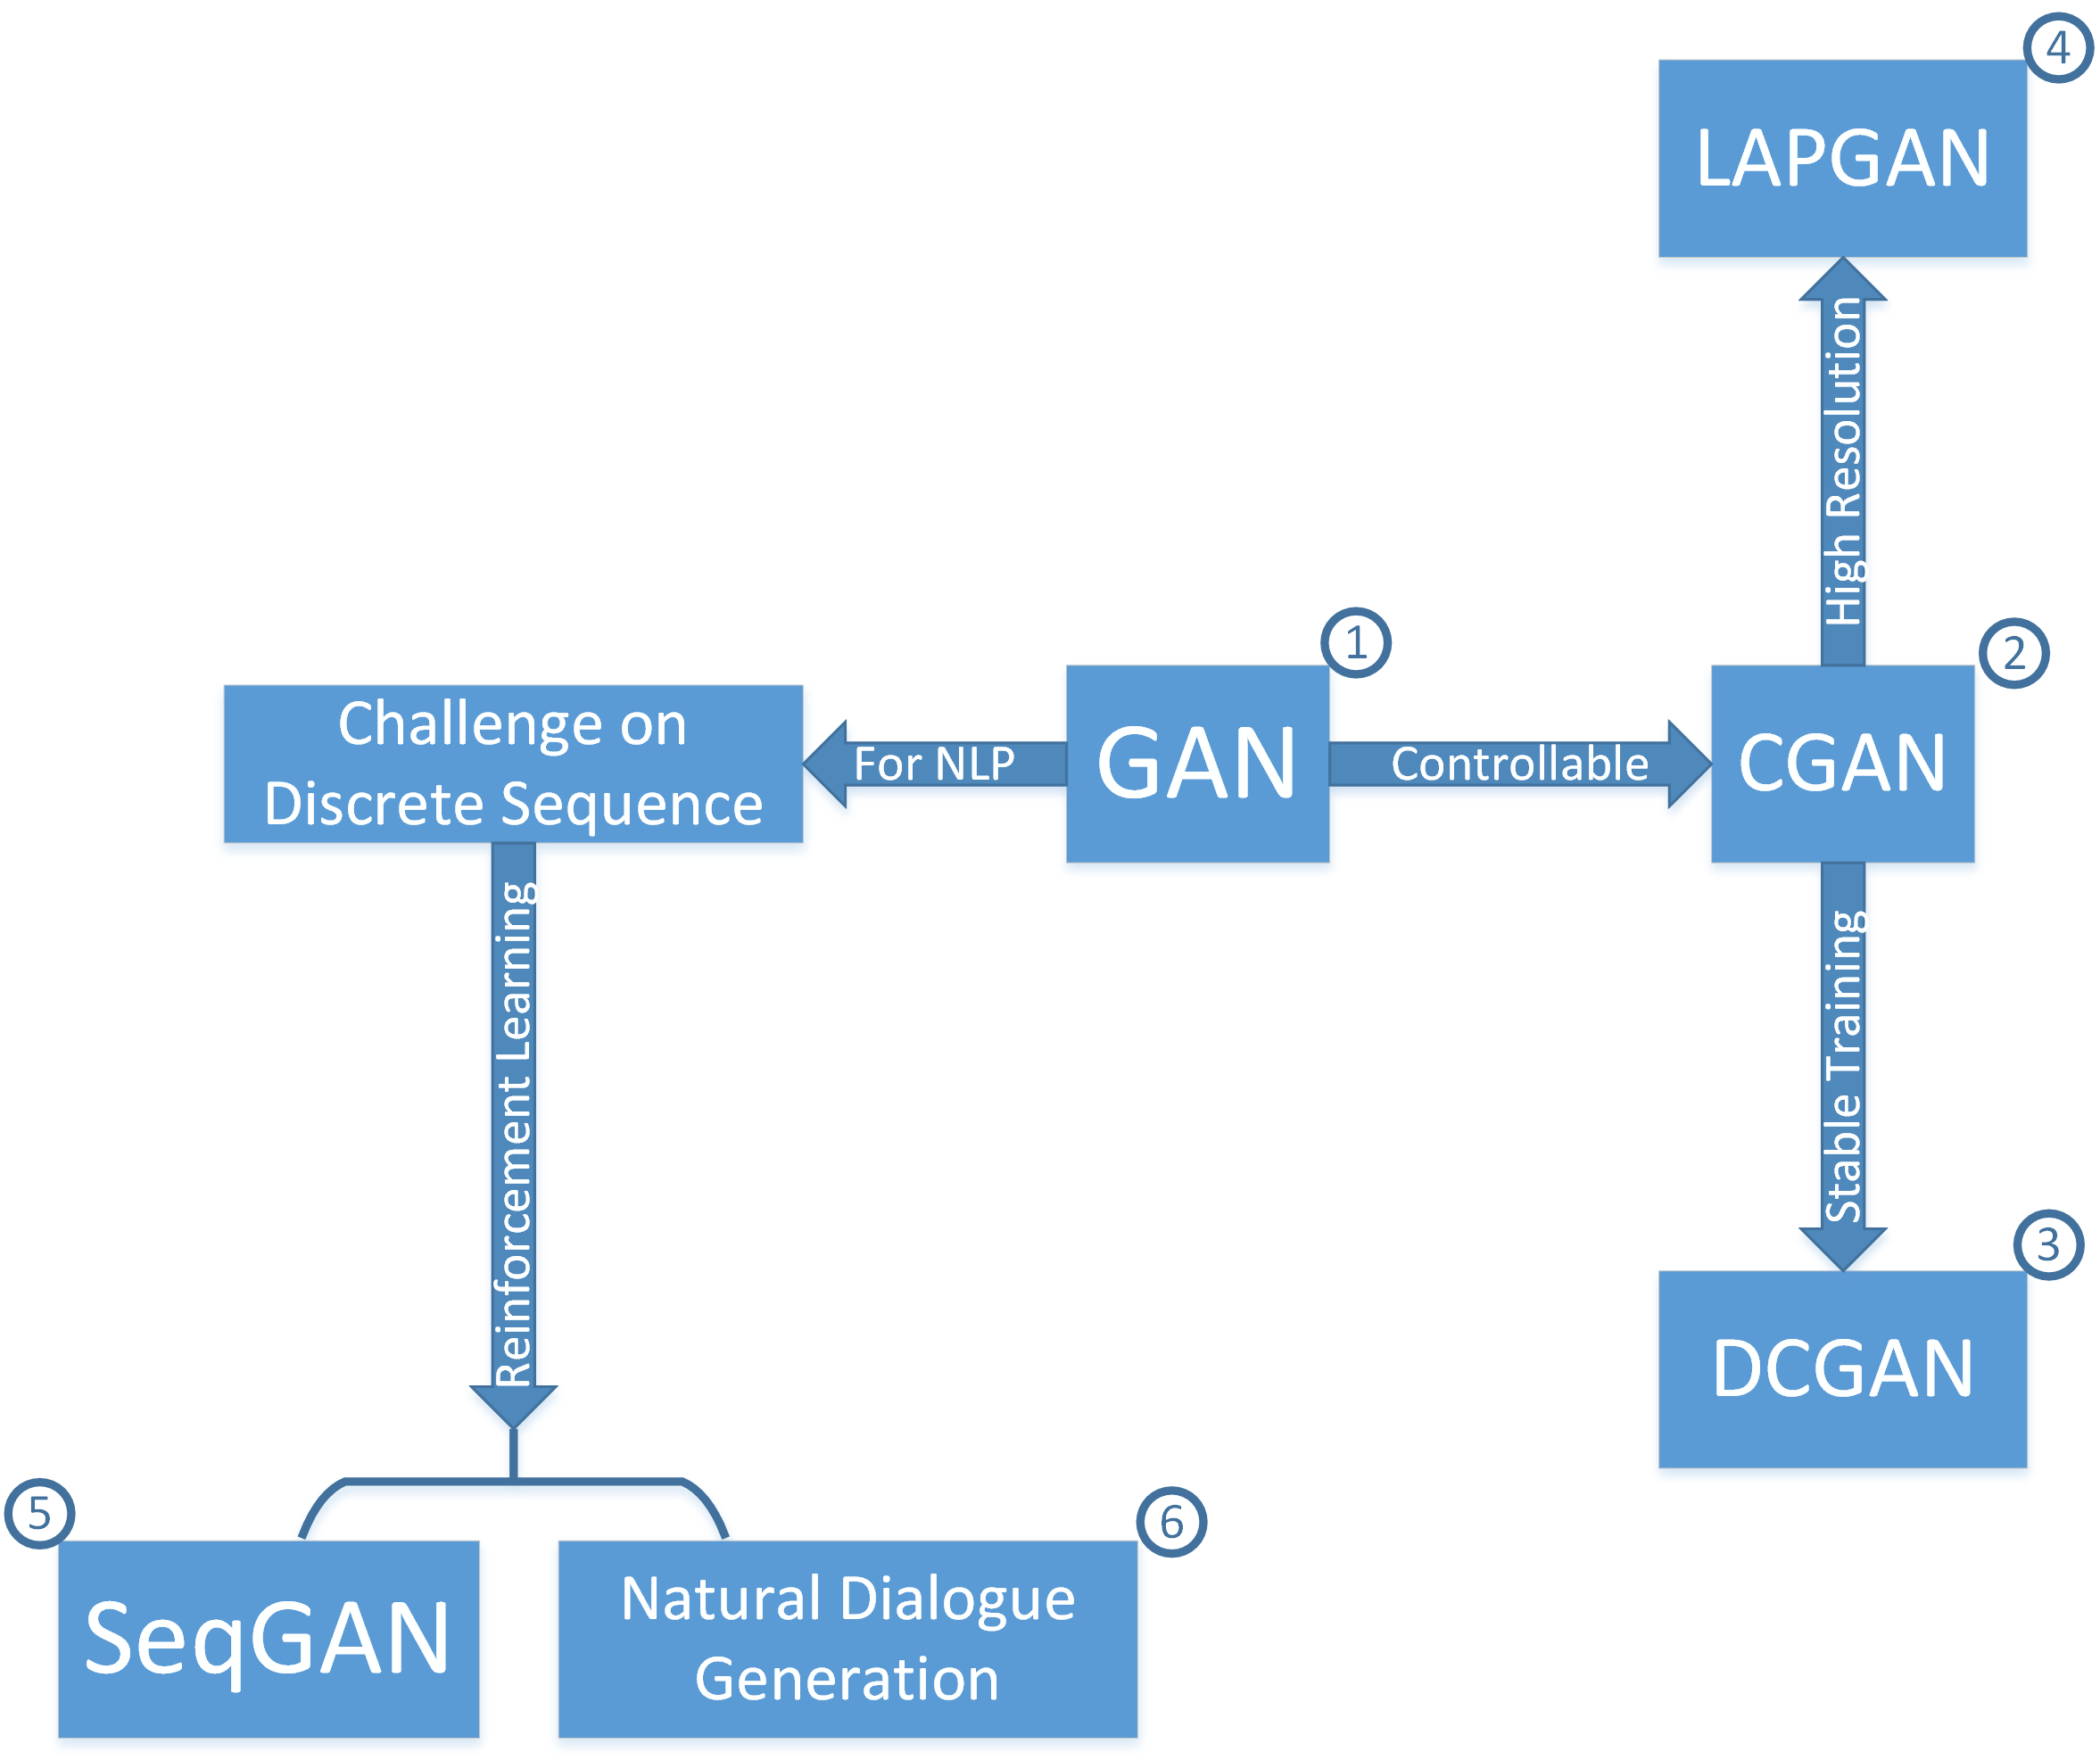
\includegraphics[width=25em]{figures/outline.png}
		\end{figure}
	\end{frame}
	\subtitlepage{}{Unsupervised Representation Learning with Deep Convolutional Generative Adversarial Networks}{Alec Radford, Luke Metz, Soumith Chintala\\arXiv: 1511.06434}
	\begin{frame}{Introduction}
		\begin{itemize}
			\item Shortcoming of GANs:
			\begin{itemize}
				\item unstable to train
				\item result ing generators that produce nonsensical outputs.
			\end{itemize}
			\item Very limited published research in trying to understand and visualize what GANs learn, and the intermediate representations of multi-layer GANs.
			\item Contributions of this paper:
			\begin{itemize}
				\item a set of constraints -> stable to train.
				\item trained discriminators for image classification task -> competitive performance.
				\item visualize the filters -> show that the filters learns to draw objects.
				\item vector arithmetic properties -> semantic manipulation.
			\end{itemize}
		\end{itemize}
	\end{frame}

	\begin{frame}{Approach}
		\begin{itemize}
			\item Architecture guidlines for stable Deep Convolution GANs:
			\begin{itemize}
				\item Replace any pooling layers with strided convolutions (discriminator) and fractional-strided convolutions (generator).
				\item Use batch normalization in both the generator and the discriminator.
				\item Remove fully connected hidden layers for deeper architectures.
				\item Use ReLU activation in generator for layers except for the output. which uses Tanh.
				\item Use LeakyReLU activation in the discriminator for all layers.
			\end{itemize}
		\end{itemize}
	\end{frame}

	\begin{frame}{Structure}
		\begin{figure}
			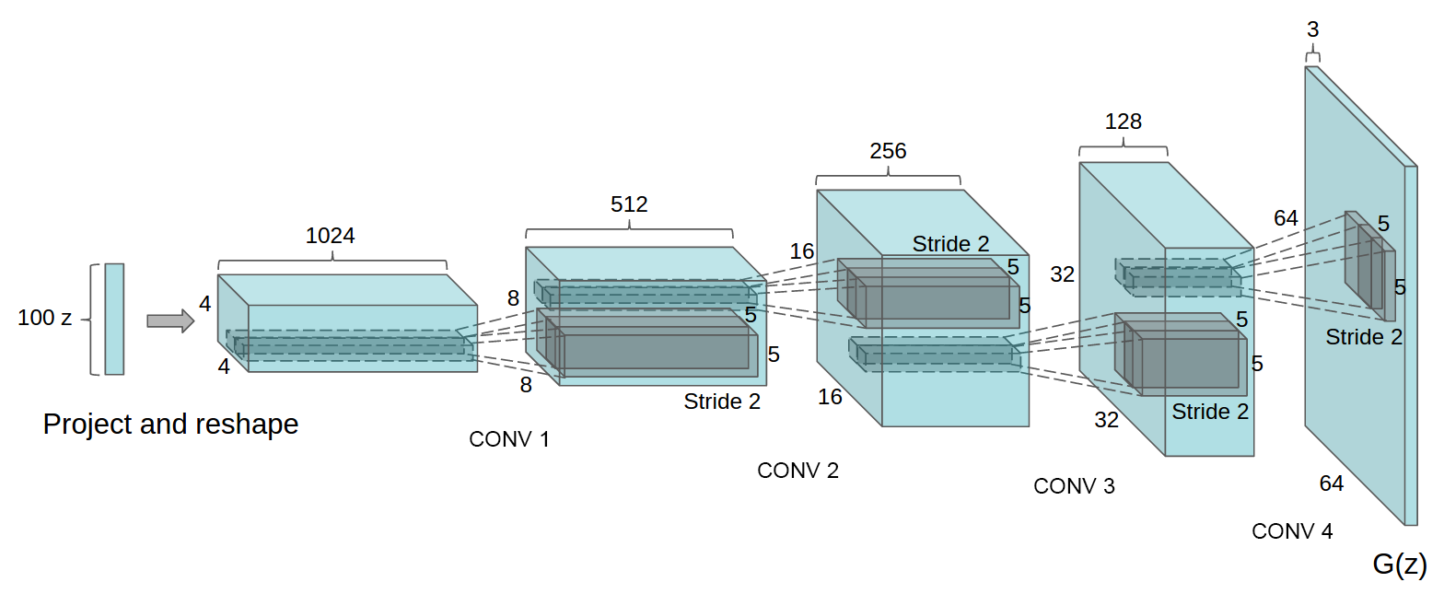
\includegraphics[width=25em]{figures/DCGAN-generator-structure.png}
			\caption{DCGAN generator used for LSUN scene modeling.}
		\end{figure}
		During the training, many technics are adopted including dropout and momentum.
	\end{frame}

	\begin{frame}{Experiment}
		\begin{figure}
			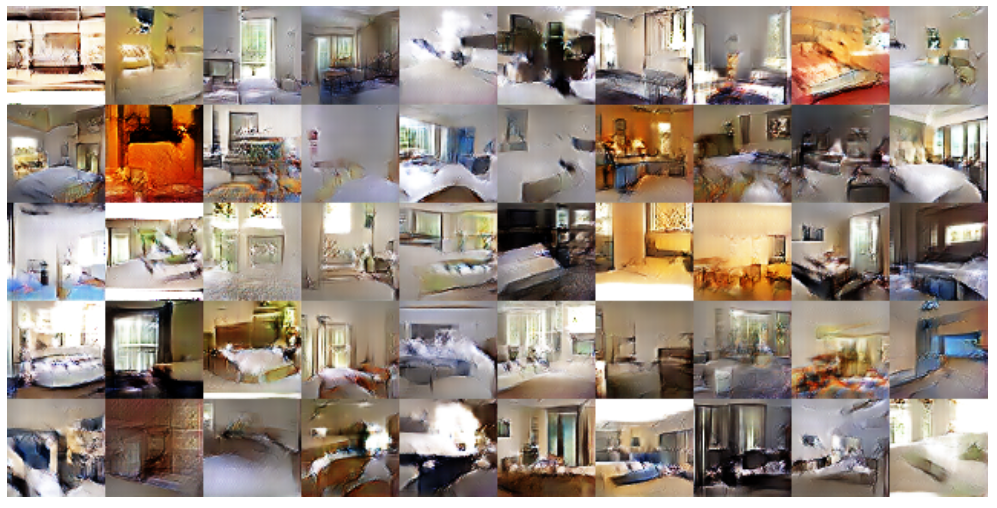
\includegraphics[width=23em]{figures/DCGAN-generated-image-epoch-1.png}
		\end{figure}
		\vspace{-1.5em}
		\begin{figure}
			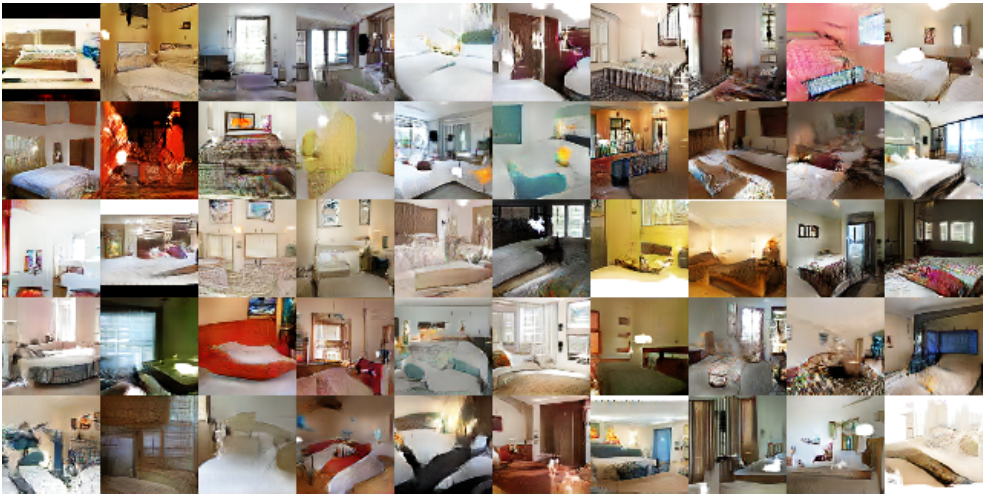
\includegraphics[width=23em]{figures/DCGAN-generated-image-epoch-5.png}
		\end{figure}
	\end{frame}

	\begin{frame}{Empirical Validation of DCGANs Capabilities}
		\begin{itemize}
			\item Classifying CIFAR-10 using GANs as a Feature Extractor
			\item To evaluate the quality of the representations learnt by DCGANs for supervised tasks:
			\begin{itemize}
				\item the model was trained on ImageNet-1k.
				\item use the discriminator's convolutional features from all layers.
				\item maxpooling each layers representation to produce a $4\times 4$ spatial grid.
				\item flattened and concatenated to form a 28672 dimensional vector.
			\end{itemize}
			\begin{figure}
				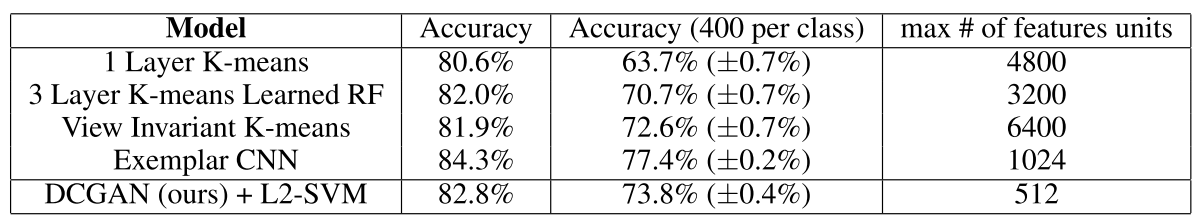
\includegraphics[width=30em]{figures/DCGAN-discriminator-feature-extractor-cifar-10.png}
			\end{figure}
		\end{itemize}
	\end{frame}

	\begin{frame}{Empirical Validation of DCGANs Capabilities}
		\begin{itemize}
			\item for StreetView House Numbers dataset (SVHN)
			\begin{figure}
				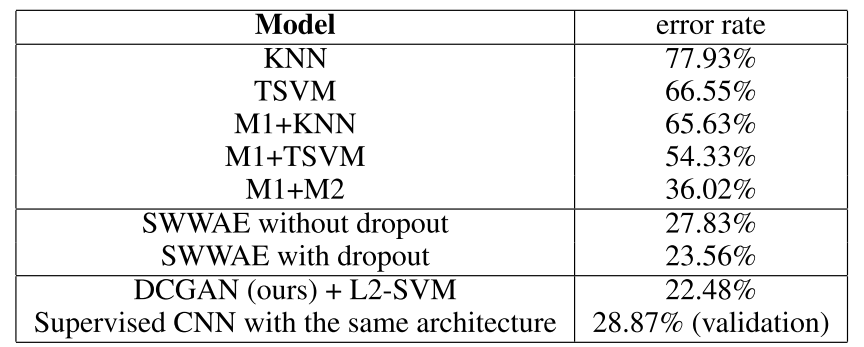
\includegraphics[width=15em]{figures/DCGAN-discriminator-feature-extractor-svhn.png}
			\end{figure}
			\item L2-SVM classifier on the top of same feature extraction extraction pipeline used for CIFAR-10.
			\item Achieves state of the art (for classification using 1000 labels) at 22.48\% test error.
			\item Additionally, authors trained a purely supervised CNN with the same architecture on the same data -> CNN architecture used in DCGAN is not the key contributing factor of the model's performance.
		\end{itemize}
	\end{frame}

	\begin{frame}{Investigating and Visualizing the Internals of the Networks}
		\begin{itemize}
			\item How to prove that the model learned feature representation instead of the mapping from a noise to a sample?
			\item If model learned the semantic representation, we can conduct small image transforms on feature space.
			\item The first experiment was to understand the landscape of the latent space.
			\item If walking in this latent space results in semantic changes to the image generations (such as object being added and removed), we can reason that the model has learned relevant and interesting representations.
		\end{itemize}
	\end{frame}

	\begin{frame}{Investigating and Visualizing the Internals of the Networks}
		\begin{figure}
			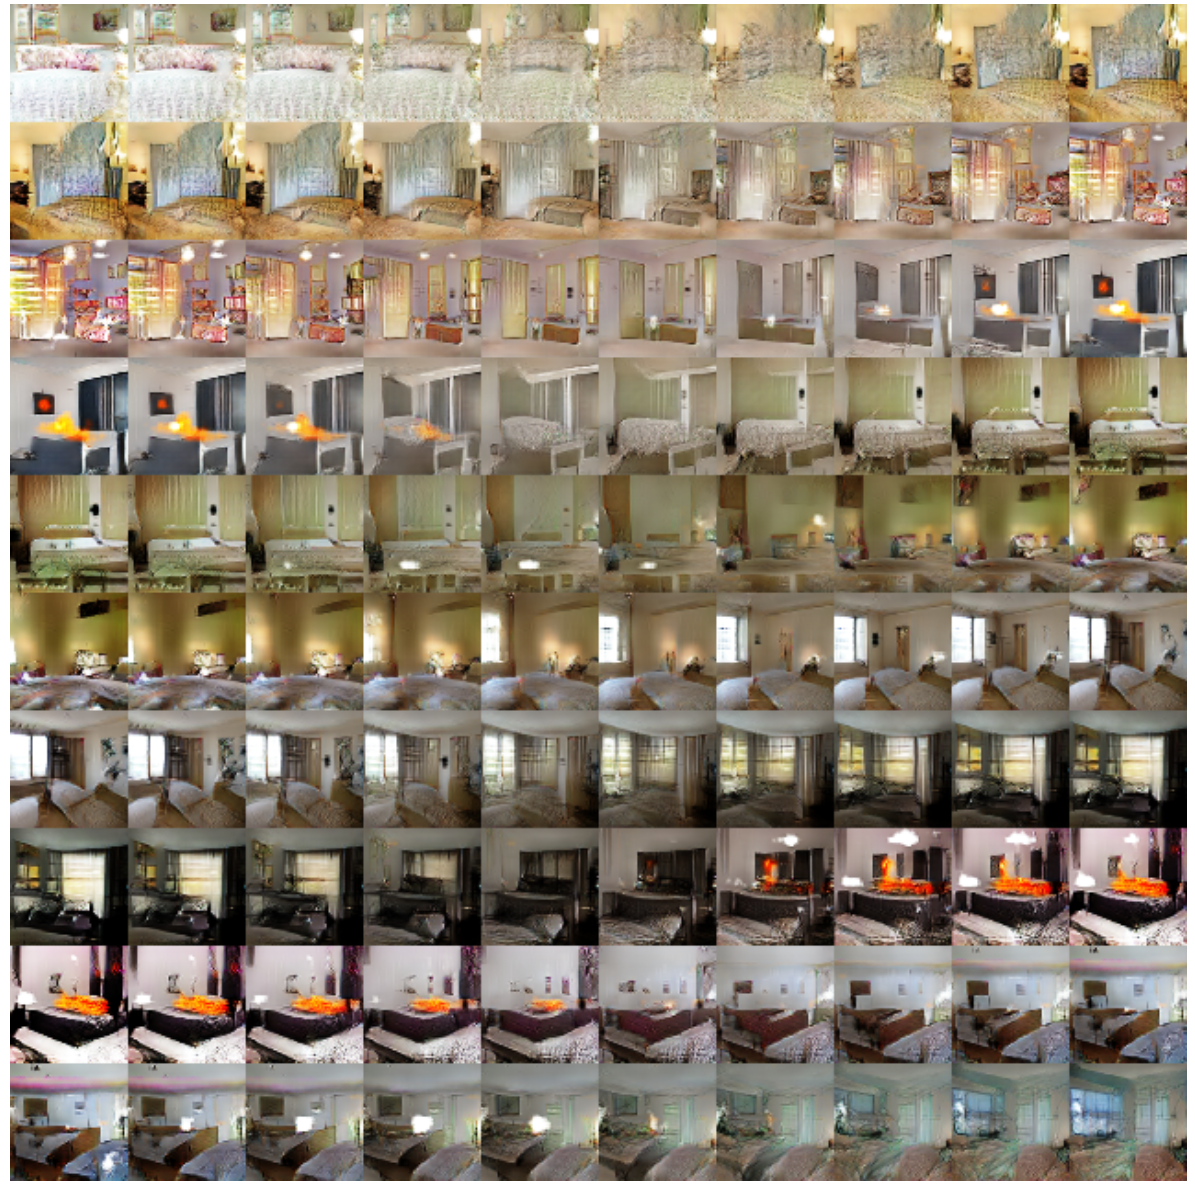
\includegraphics[width=23em]{figures/DCGAN-visualizing-internals-walking-in-latent.PNG}
		\end{figure}
	\end{frame}

	\begin{frame}{Investigating and Visualizing the Internals of the Networks}
		\begin{itemize}
			\item Unsupervised DCGAN trained on a large image dataset can also learn a hierarchy of features that are interesting.
			\begin{figure}
				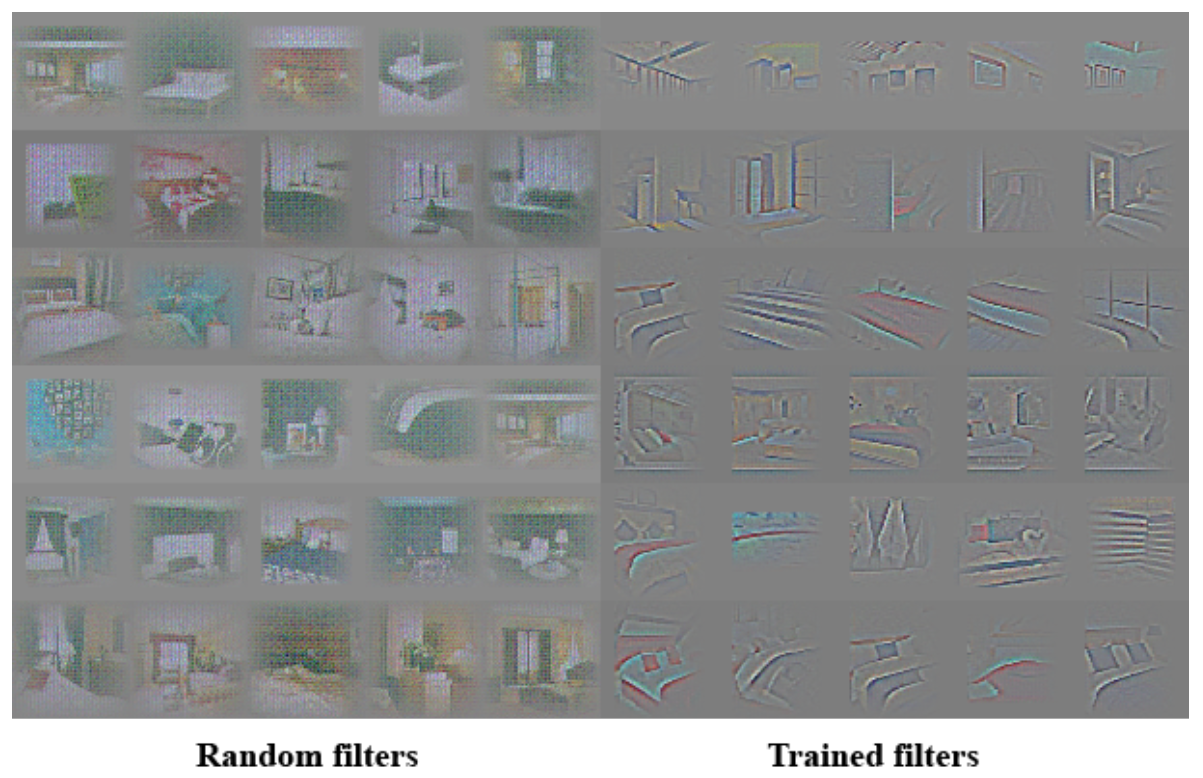
\includegraphics[width=25em]{figures/DCGAN-visualizing-internals-filters.png}
				\caption{Features learnt by the discriminator.}
			\end{figure}
		\end{itemize}
	\end{frame}

	\begin{frame}{Investigating and Visualizing the Internals of the Networks}
		\begin{itemize}
			\item Manipulating the generator representation: Forgetting to draw certain objects
			\item What representations the generator learns? Scene components? Beds? Windows? Lamps? Doors?
			\item If so, we can attempt to remove some component by manipulating the latent representation:
			\begin{itemize}
				\item 150 samples, 52 window bounding boxes were drawn manually.
				\item On the second highest convolution layers features, logistic regression was fit to predict whether a feature activation was on a window (or not).
				\item by using the criterion that activations inside the drawn bounding boxes are positive and random samples from the same images are negatives.
				\item All feature maps with weights greater than zero (200 in total) were dropped from all spatial locations.
				\item Then, random new samples were generated with and without the feature map removal.
			\end{itemize}
		\end{itemize}
	\end{frame}

	\begin{frame}{Investigating and Visualizing the Internals of the Networks}
		\begin{figure}
			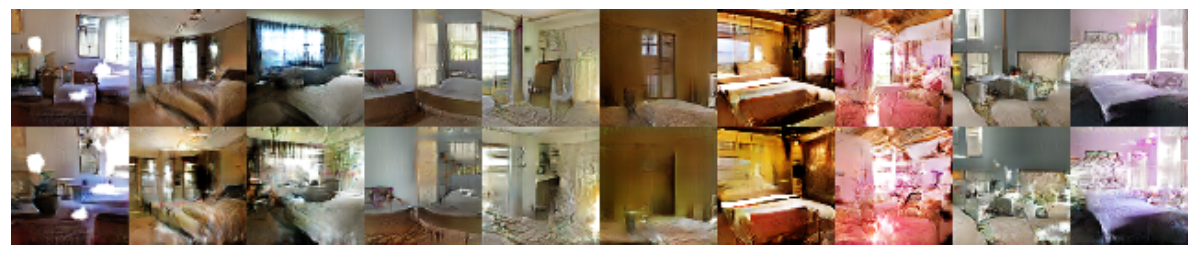
\includegraphics[width=30em]{figures/DCGAN-visualizing-internals-remove-filter.png}
		\end{figure}
		\begin{itemize}
			\item Top row: un-modified samples from model.
			\item Bottom row: the same samples generated with dropping out "window" filters.
			\item Some windows are removed, others are transformed into objects with similar visual appearance such as doors and mirrors.
		\end{itemize}
	\end{frame}
	
	\begin{frame}{Investigating and Visualizing the Internals of the Networks}
		\begin{itemize}
			\item Representation of words: vector("King")-vector("Man")+vector("Woman")$\approx$vector("Queen").
			\item Similar structure emerges in the $Z$ representation of generators.
			\item Experiments working on only single samples per concept were unstable -> averaging the $Z$ vector for three examples.
			\begin{figure}
				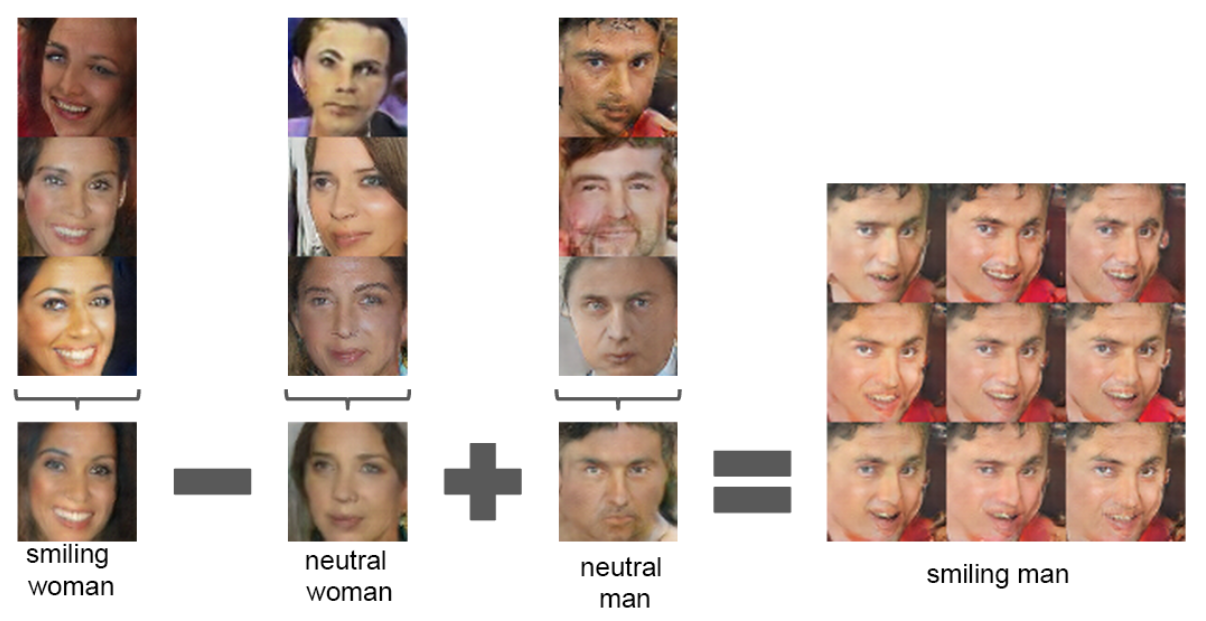
\includegraphics[width=25em]{figures/DCGAN-visualizing-internals-vector-1.PNG}
			\end{figure}
		\end{itemize}
	\end{frame}

	\begin{frame}{Investigating and Visualizing the Internals of the Networks}
		\begin{figure}
			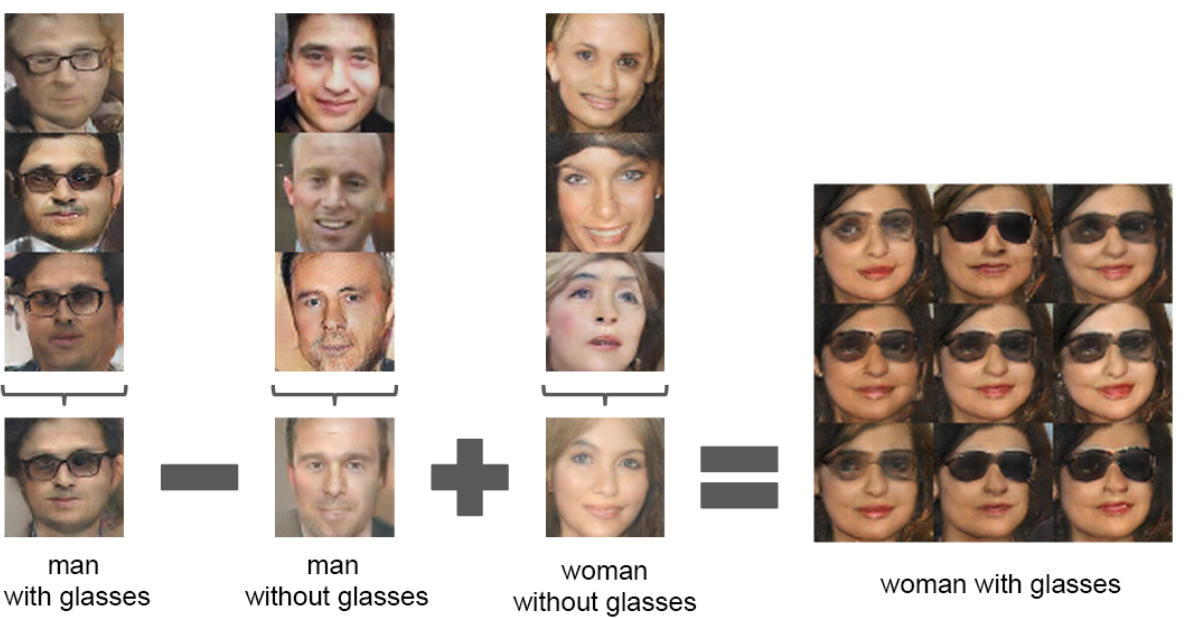
\includegraphics[width=25em]{figures/DCGAN-visualizing-internals-vector-2.PNG}
		\end{figure}
	\end{frame}

	
	\part{LAPGAN}
	\part{Challenge On NLP}
	\part{Background: Reinforcement Learning and Policy Gradient}
	\part{SeqGAN}
	\part{Neural Dialogue Generation}
\end{document}